\chapter{Realizacja projektu}
\label{cha:realizacja}

Realizacja projektu została podzielony na kilka etapów w których każdy jest zależna od  poprzedniego. Najważniejszymi etapami są: teoretyczne przygotowanie do zagadnienia wraz z doborem topologii sieci, implementacja algorytmu w środowisku MATLAB wraz z algorytmem uczenia sieci oraz ostateczna jego realizacja na układzie fpga. 
\section{Dobór topologii sieci}

Wybór odpowiedniej topologii sieci wymagał znajomości teoretycznej zagadnień związanych z algorytmami opartymi na sieciach neuronowych, wykorzystania własnego doświadczenia związanego z tymi zagadnieniami oraz realizacją algorytmów na układach fpga. Ze względu na niewystarczającą wiedzę w temacie sieci neuronowych, początkowa faza projektu opierała się na poszukiwaniu informacji o zagadnieniach zbliżonych do tematu projektu. Okazało się, iż bardzo zbliżony projekt został już zrealizowany i opisany w \cite{fdciuss}. Artykuł przedstawia dokładne etapy realizacji projektu którego celem było rozpoznawanie twarzy. Zawierał on również dokładny opis topologi sieci oraz sposób przygotowania danych do przetwarzania. 

Informacje te okazały się bardzo pomocne, pozwoliły one rozpocząć doświadczalny dobór topologi sieci, która pozwoli na poprawne przetwarzanie danych wejściowych. 
Podstawą do przeprowadzania takich eksperymentów było zdobycie bazy (została ona załączona wraz z plikami projektu), która umożliwi naukę sieci. Baza posiada zbiór danych przygotowany w formie 4 wartości odpowiadających poszczególnym wartością RGB oraz oczekiwanemu wyjściu z sieci, którego wartości zamykają się w zbiorze \{0,1\}. Świadczy ono o tym czy na podstawie określonego wejścia powinna zostać wykryta skóra.

Liczna baza danych wypełniona powyżej opisanymi rekordami pozwoliła na przeprowadzanie pierwszych doświadczeń. Na podstawie zdobytych zauważono, iż jakość wykrywania pikseli przedstawiających skórę znacznie wzrasta jeśli na wejście sieci oprócz sygnałów RGB podawane zostaną również CbCr(wartości sygnałów z modelu przestrzeni kolorów YCbCr) oraz HS(wartości sygnałów z przestrzeni barw HSV). Aby otrzymać pełny wektor danych wejściowych zaimplementowano algorytm w postaci skryptu w programie MATLAB, który na podstawie wartości RGB wyznaczał pozostałe parametry. Tak przygotowane dane wejściowe podawano na wejście wbudowanej sieci neuronowej w środowisko MATLAB, a następnie na podstawie przykładowego zdjęcia określano czy sieć poprawnie rozpoznaje skórę na przedstawionym obrazie. Ze względu na łatwą konfigurację topologii sieci sposób ten umożliwił szybkie przetestowanie wielu wariantów oraz wybranie najlepszego w interesującym nas zakresie.

\begin{figure}[tbph!]
	\centering
	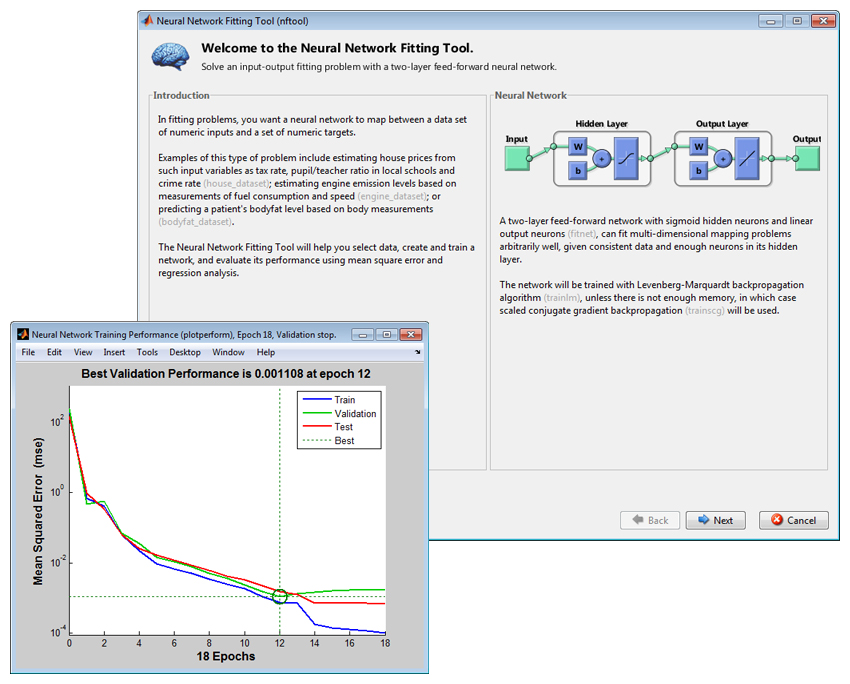
\includegraphics[width=0.9\linewidth]{images/matlabnn.jpg}
	\caption{Narzędzie środowiska MATLAB służące do testów sieci neuronowych}
	\label{fig:nnmatlab}
\end{figure}

Najlepsze rezultaty uzyskaliśmy dla sieci posiadającej 7 wejść, 13 neuronów w warstwie ukrytej oraz jednym w warstwie wyjściowej. Niestety narzędzie to uniemożliwia konfigurowanie funkcji wyjścia z neuronu. Na podstawie doświadczeń, zaimplementowanych skryptów oraz zdobytej wiedzy udało się rozpocząć prace nad kolejnym etapem.

\section{Implementacja sieci neuronowej w MATLAB}
\label{cha:impl-MATLAB}
W tej fazie skoncentrowano się na implementacji sieci spełniającej nasze wymagania. Ze względu na prostotę działania wybraliśmy sieci propagation o strukturze wybranej w poprzednim etapie czyli. 7 wejść, 13 neuronów w warstwie ukrytej oraz 1 wyjściu.

Model takiej sieci zakłada prosty przepływ informacji miedzy kolejnymi warstwami, neurony w warstwie wejściowej przekazują wartość na wejścia neuronów w warstwie ukrytej.
Następnie są one przemnażana przez wartość wagi przypisane do wejścia na którym się pojawiła. Wartości te są sumowane w obrębie każdego z neuronów, a następnie przekazywane na wyjście, które ostatecznie na otrzymanej wartości wywołuje funkcje przejścia. Jednoznacznie określona wartość wyjścia przekazywana jest do następnej warstwy (przepływ danych przez sieć przedstawiono na rysunku \ref{fig:nn}).

\begin{figure}[tbph!]
	\centering
	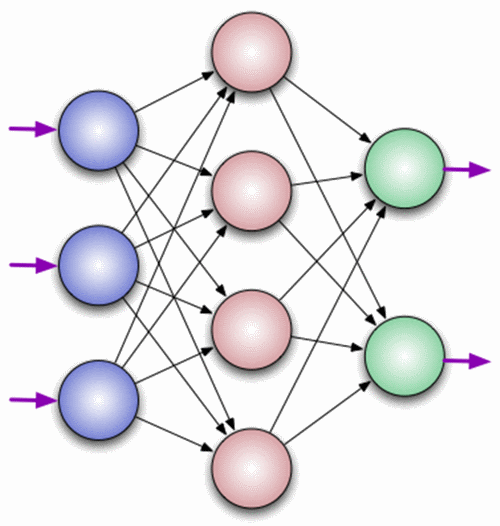
\includegraphics[width=0.7\linewidth]{images/nn.png}
	\caption{Sieć neuronowa typu propagation.}
	\label{fig:nn}
\end{figure} 

W tym przypadku stosowanie sieci o bardziej złożonych strukturach wydaje się zbędny i sprzeczny z intuicją. Sieci te doskonale rozpoznają cechy wartości podanych na wejście co powoduje poprawne zachowanie również dla sygnałów zbliżonych z którymi sieć nie miała wcześniej styczności. 

Ważną cechą sieci jest dobór funkcja przejścia dla neuronów. W tym przypadku została zastosowana funkcja $tanh(x)$ ze względu na jej charakterystykę, która akcentuje wartości brzegowe. W omawianym przypadku odpowiadają wykryciu skóry przez sieć. 

Po implementacji sieci przystąpiono do adaptacji algorytmu uczenia. W sieciach typu propagation najczęsciej stosowany jest algorytm backpropagation, który cechuje się prostą lecz również żmudnymi obliczeniami oraz długimi czasami uczenia sieci. Polega on na podawaniu na wejście sieci wektor odpowiednich wartości, a następnie wyznaczaniu różnicy wyjścia sieci z wartością oczekiwaną. Różnica ta jest przetwarzana wstecznie przez sieć wraz z wyznaczaniem gradientów błędów poszczególnych neuronów. Na ich podstawie korygowane są wagi każdego z wejść neuronów co powoduje uczenie sieci.

Wszystkie skrypty utworzone na tym etapie oraz obszerna baza danych umożliwiły rozpoczęcie prac nad uczeniem sieci. Wywołanie odpowiednich skryptów rozpoczynało proces uczenia sieci, którego czas trwania zależał od ilości wykonania powyżej opisanej operacji dla każdego z wierszy. Optymalne wyniki otrzymane były dla około 100 iteracji dla każdego elementu z bazy danych. Warto również wspomnieć, iż początkowo baza zawierała dane posortowane ze względu na wektor oczekiwanego wyjścia co zdecydowanie utrudniało proces uczenia. Rozwiązano ten problem przez przemieszanie wierszy w bazie.

Na rysunku \ref{fig:reka} przedstawiono przykładowe przetworzenie małego obrazka na którym testowano sieć po zakończeniu uczenia. Na jego podstawie wstępnie oceniano powodzenie procesu uczenia sieci. Jak widać na rysunku udało się osiągnąć zadowalającą jakość. Warto zauważyć, iż zdjęcie testowe zostało wykonane przez autorów projektu więc wartości RGB poszczególnych pikseli są niezależne względem tych umieszczonych w bazie.

\begin{figure}[tbph!]
	\centering
	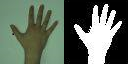
\includegraphics[width=0.6\linewidth]{images/reka.png}
	\caption{Przykładowy wynik testu działania sieci po uczeniu.}
	\label{fig:reka}
\end{figure}

W kolejnej fazie zmodyfikowano system reprezentacji liczb na których bazuje działanie sieci neuronowej. Zastosowano zmienne typu fixed\_point, które pozwalają na dokładne określenie ilości bitów przeznaczonych na reprezentacje poszczególnej liczby. Do konwersji z typu double do typu fixed\_point został stworzona funkcja w środowisku MATLAB. Jako argument przyjmuje ona zmienną typu double, a następnie na podstawie sztywno określonej konfiguracji funkcji tworzy zmienną typu fixed\_point, która reprezentuje wartość argumentu lub wartość zbliżoną, która jest możliwa do zaprezentowania. Zabieg ten miał na celu dokładne odwzorowanie działania sieci na układzie fpga. Czas przetwarzania obrazu testowego przez sieć, a w szczególności sam proces uczenia wydłużył się kilkakrotnie ze względu na liczne konwersje.

Po przeprowadzaniu ponownego procesu uczenia oraz sprawdzeniu, że modyfikacje te nie zaburzyły w znaczny sposób działania zakończono proces tworzenia odwzorowania sieci w środowisku MATLAB. 

Podczas realizacji tej fazy zorientowano się, iż właściwa implementacja na układzie fpga nie wymaga implementowania procesu uczenia co zdecydowanie upraszcza implementacje. Uzyskane dotychczas informacje na temat topologii sieci, funkcji przejścia, wartości poszczególnych wag dla każdego z neuronów oraz optymalnej ilości bitów przeznaczonych do reprezentacji tych wartości pozwoliły na przystąpienie do ostatniego etapu.

\section{Realizacja algorytmu w środowisku ISE}

Implementacja algorytmu w środowisku ISE opierała się na modyfikacjach programu wykonanego w poprzednim semestrze, dokładny opis wraz z tutorialem znajduje się znajduję się w \cite{skryptFPGA}. Pomimo tego, tor wizyjny należało rozwinąć o dwa istotne i najbardziej skomplikowane elementy: 

\begin{itemize}
\item Moduł przenoszący sygnał z przestrzeni RGB do przestrzeni HSV.
\item Moduł klasyfikujący każdy piksel jako \textit{skóra} lub \textit{nie-skóra} i binaryzujący na tej podstawie obraz.
\end{itemize}


Uproszczony schemat logiki całego systemu jest przedstawiony na diagramie \ref{fig:schema1}. 

\begin{figure}[tbph!]
	\centering
	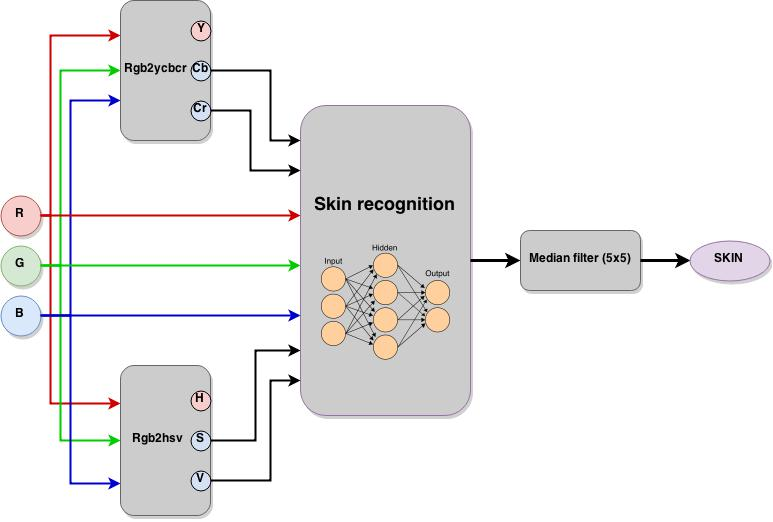
\includegraphics[width=1.1\linewidth]{images/schema1.jpg}
	\caption{Uproszczony schemat logiki całego systemu.}
	\label{fig:schema1}
\end{figure}

\subsubsection{Konwersja RGB -> HSV}

Konwersja z przestrzeni sygnału z przestrzeni RGB do przestrzeni HSV została zrealizowana dokładnie według opisu zadania dodatkowego w \cite{skryptFPGA}.

\subsubsection{Wykrywanie skóry (binaryzacja)} 

Moduł \textit{Skin recognition} jest implementacją sieci neuronowej opisanej w \ref{cha:impl-MATLAB}.

 Opiera się on na odpowiednio połączonych modułach neuronów  (zaprezentowanych na schemacie \ref{fig:neuron}) warstwy ukrytej oraz wyjściowej.

\begin{figure}[tbph!]
	\centering
	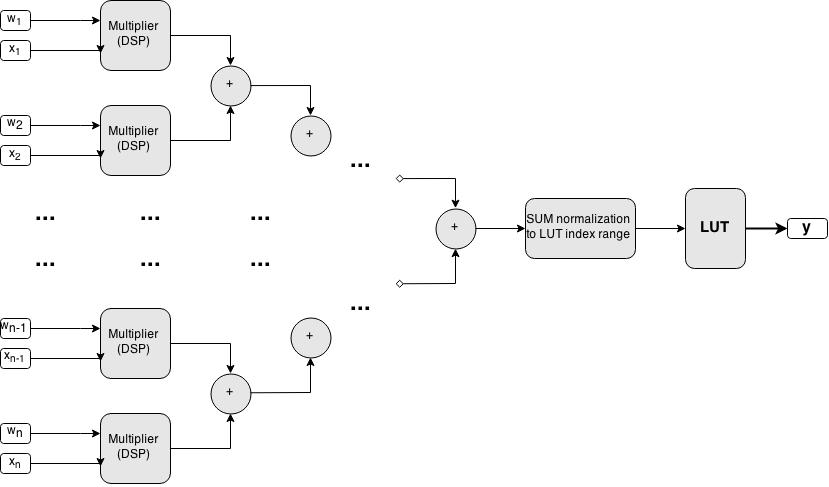
\includegraphics[width=1.1\linewidth]{images/wsw-neuron.jpg}
	\caption{Uproszczony schemat logiki zaimplementowanego neuronu.}
	\label{fig:neuron}
\end{figure}


\subsubsection{Uwagi} 
\begin{itemize}

\item Niestety z powodu błędnego podpięcia sygnałów do filtru medianowego nie działał on poprawnie podczas ostatecznego testu.
\item Po zaimplementowaniu całego systemu zauważono, że układ \textbf{Spartan-6} posiada za mało zasobów i cała logika została przeniesiona na układ \textbf{Virtex-7}.
\item Zgodnie z założeniami, wartości wejściowe zawierały się w zakresie \textit{[0,255]} i powinny zostać znormalizowane do zakresu\textit{ [0,1]}, co miało być zrealizowane przy pomocy dzielenie każdej wartości przez \textit{255}. Jednak aby zmniejszyć wykorzystanie zasób postanowiliśmy dzielić wartości przez \textit{256} (przesunięcie bitowe), co w żaden sposób nie pogorszyło otrzymywanych rezultatów.
\item Kod odpowiadający wagą każdego z neuronów generowano przy pomocy napisanego skryptu w MATLABie i był wklejany jako stałe wartości rejestrów. 
\item Funkcja przejścia została zrealizowana przy pomocy tablicy LUT, a jej wartości w formie binarnej również były generowane przy pomocy napisanego skryptu i wklejane do odpowiedniego pliku.
\item Próg końcowy został ustalony jako wartość stała równa \textit{0.3}.
\item Dobrym pomysłem rozwinięcia projektu byłaby implementacja komunikacji UART umożliwiająca zmianę wyżej wymienionych stałych wartości w trakcie działania systemu.
\item Dzięki zręcznie zdefiniowanym sygnałom była możliwa generacja mnożarek oraz część drzew sumacyjnych przez wykorzystanie instrukcji \textit{generate} w każdym neuronie, umożliwiło to znaczne uproszczenie kodu i przyśpieszyło nanoszenie wszelkich poprawek.

\end{itemize}
